

\textbf{Problem 1:}

Let us assume that the controller has been designed (or optimized) with the
assumption that the delays suffered by messages is bounded by one sampling
period (i.e., this is the deadline). If certain message instances, e.g., m i , m j ,
m k , . . ., miss this deadline then this will negatively impact control performance.

However, if not too many messages miss their deadlines then the control performance
might be within the acceptable limit.
In this problem, we will specifically consider deadline misses of the following
form:
every invalid message $m_i$ is followed by at least $k$ valid messages
$m_{i+1}$, \dots $m_{i+k}$,
where a message that misses its deadline is referred to as an invalid message
and one that meets its deadline is referred to as an valid message.
Let us assume that for a certain k a given control performance requirement
is satisfied (details on this may be found in [?]).
Question (Verification): Is this $k$ satisfied by the platform?

To answer this question, we can start with a simple setup with only two processors
communicating via a bus. The bus implements a given scheduling policy
(e.g., TDMA, fixed priority, or any other), with messages from the application
at hand being scheduled with messages from other applications that are not being 
analyzed. We would like to apply model checking techniques to answer if the
given k is satisfied by the bus scheduling policy and messages to be scheduled.
This setup can then be extended to consider not only the schedule on the
bus, but also the scheduling policies on the processors.
Question (Synthesis): For a given k, can we synthesize a bus schedule such
that the platform satisfies this k?
Again, this synthesis problem may be extended to consider not only bus
schedules but also the processor schedules.

\textbf{Motivating Example:}

\begin{figure}
\begin{center}
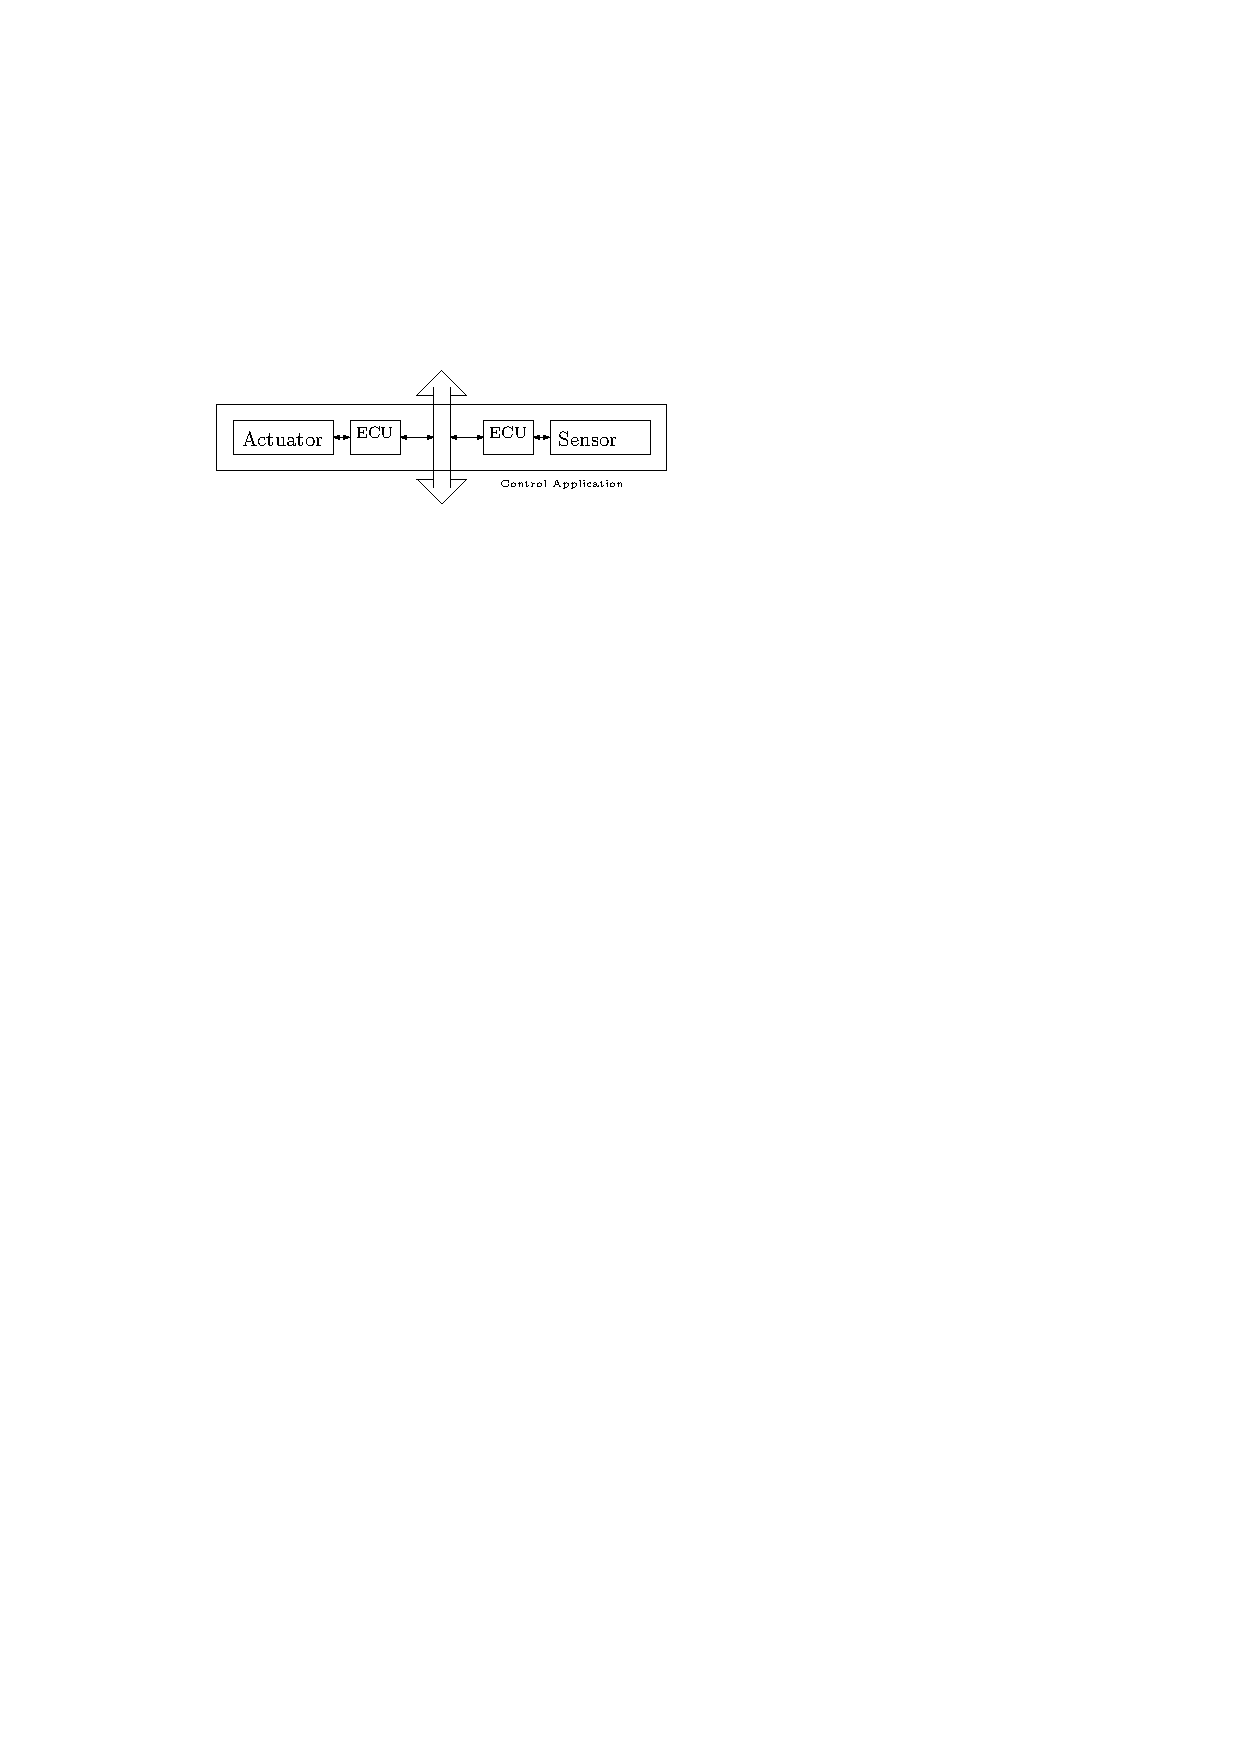
\includegraphics[width = 80mm]{system_block_diagram.pdf}
\end{center}
\caption{System Block Diagram}
\label{block_dig}
\end{figure}

The diagram of the distributed platform is given in Fig.\ref{block_dig}.
In the diagram a control application is divided into two tasks, a sensor task $T_s$ and 
an actuator task $T_a$. These tasks run on two different processors and
uses a common shared bus. A bus schedule is there to schedule messages on the bus.
When sender generates a message, it waits for the bus scheduler to get the bus
access and when bus scheduler allots bus to the message it gets transmitted to
the receiver's processor to be accessed by the receiver. Say at a particular period  
$p$, $T_a$ sends message $m_a$ to the bus and receive feedback message $m_s$ and $T_s$
accepts message $m_a$ and sends feedback message $m_s$. The timing diagram is given in Fig.\ref{tim_dig}

\begin{figure}
\begin{center}
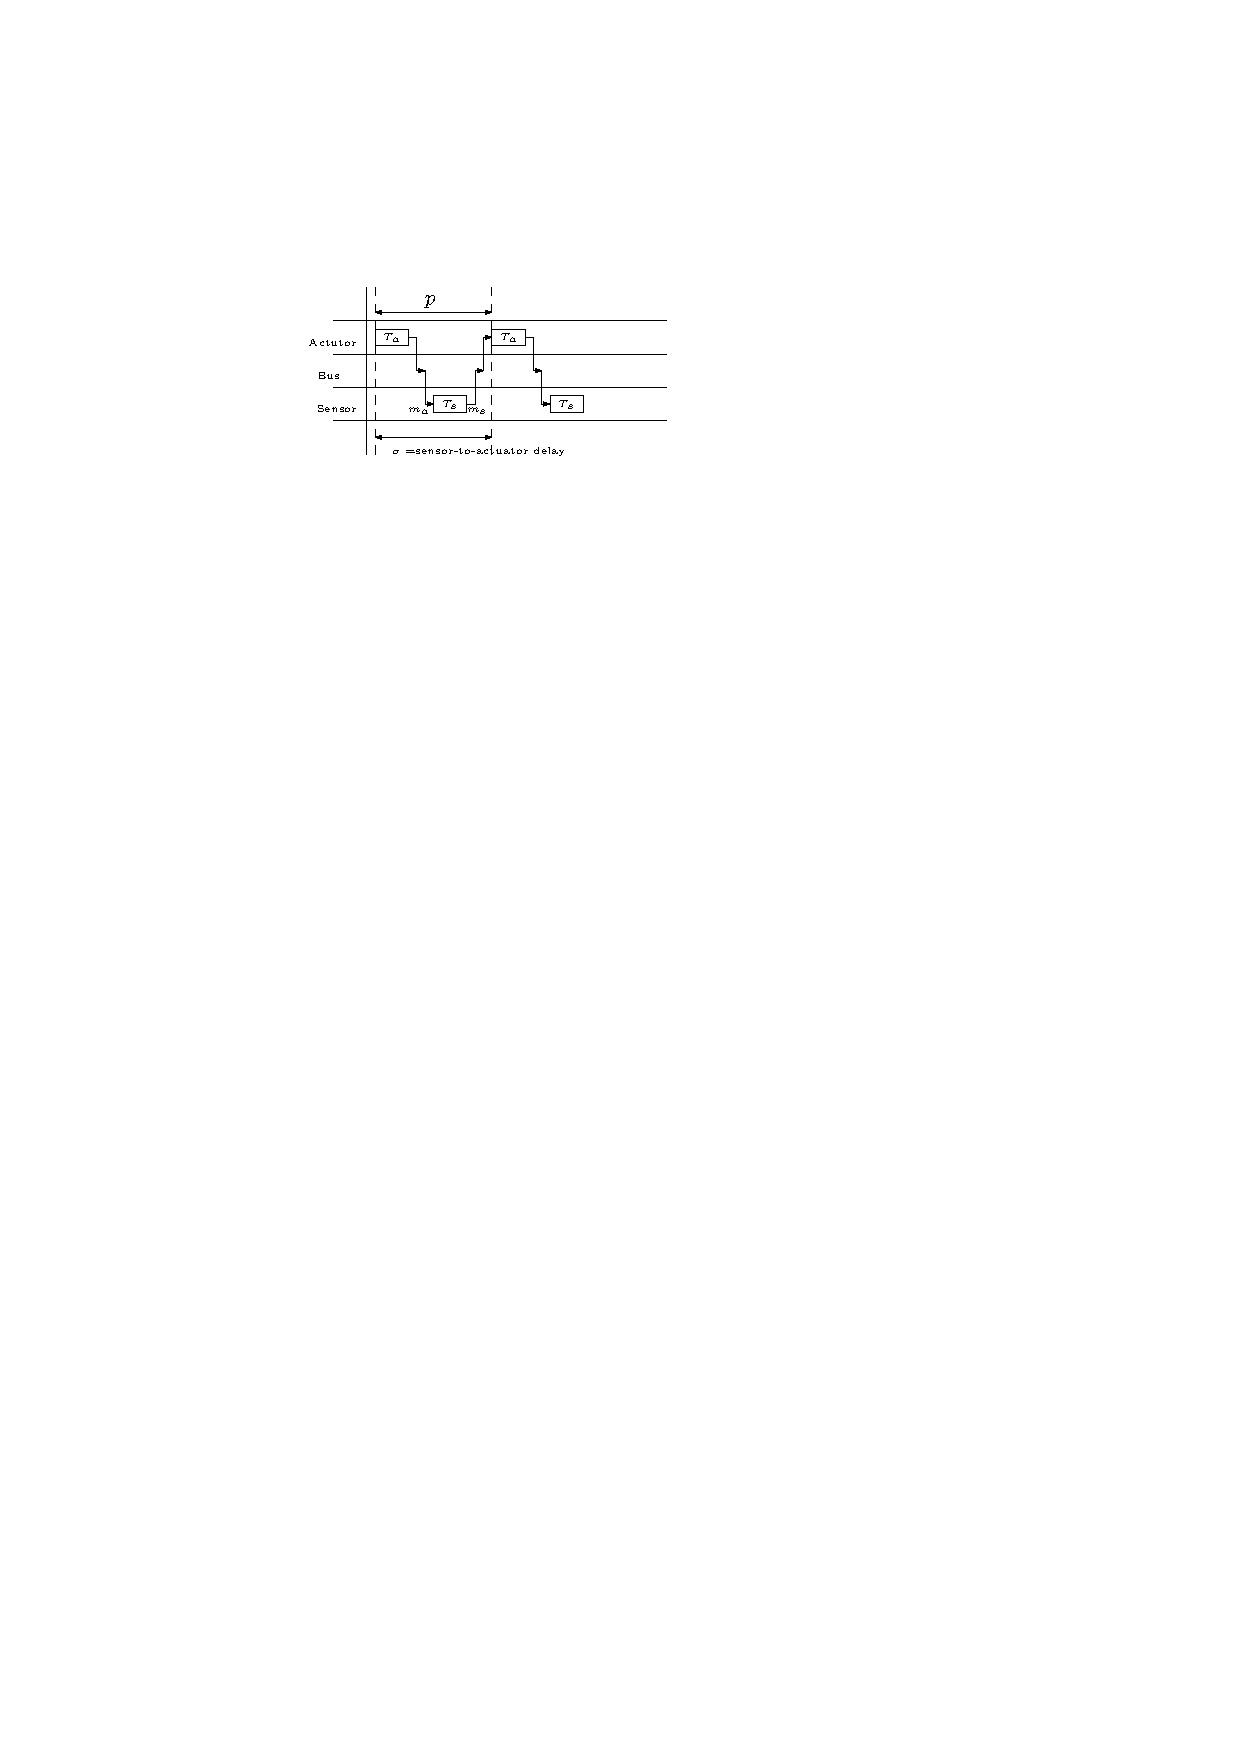
\includegraphics[width=75mm]{timing_diagram_deadline_cosntraint.pdf}
\end{center}
\caption{Timing diagram}
\label{tim_dig}
\end{figure}


The time interval between the sending message and receiving message is the
sensor-to-actuator delay denoted by $\sigma$. According to the timing diagram,
the sensor-to-actuator delay can be measured by total time needed by $T_a$
to send $m_a$ and getting feedback message $m_s$, which is some function of $m_a$,
i.e $m_s = f(m_a)$. 

From the timing diagram we can understand that $\sigma > 0$ and $\lceil{h|\sigma}\rceil >= 1$
should be true always. Such kind of constraint are common in computational process and 
control algorithms where they share a common bus in a distributed environment.


\begin{figure}
\begin{center}
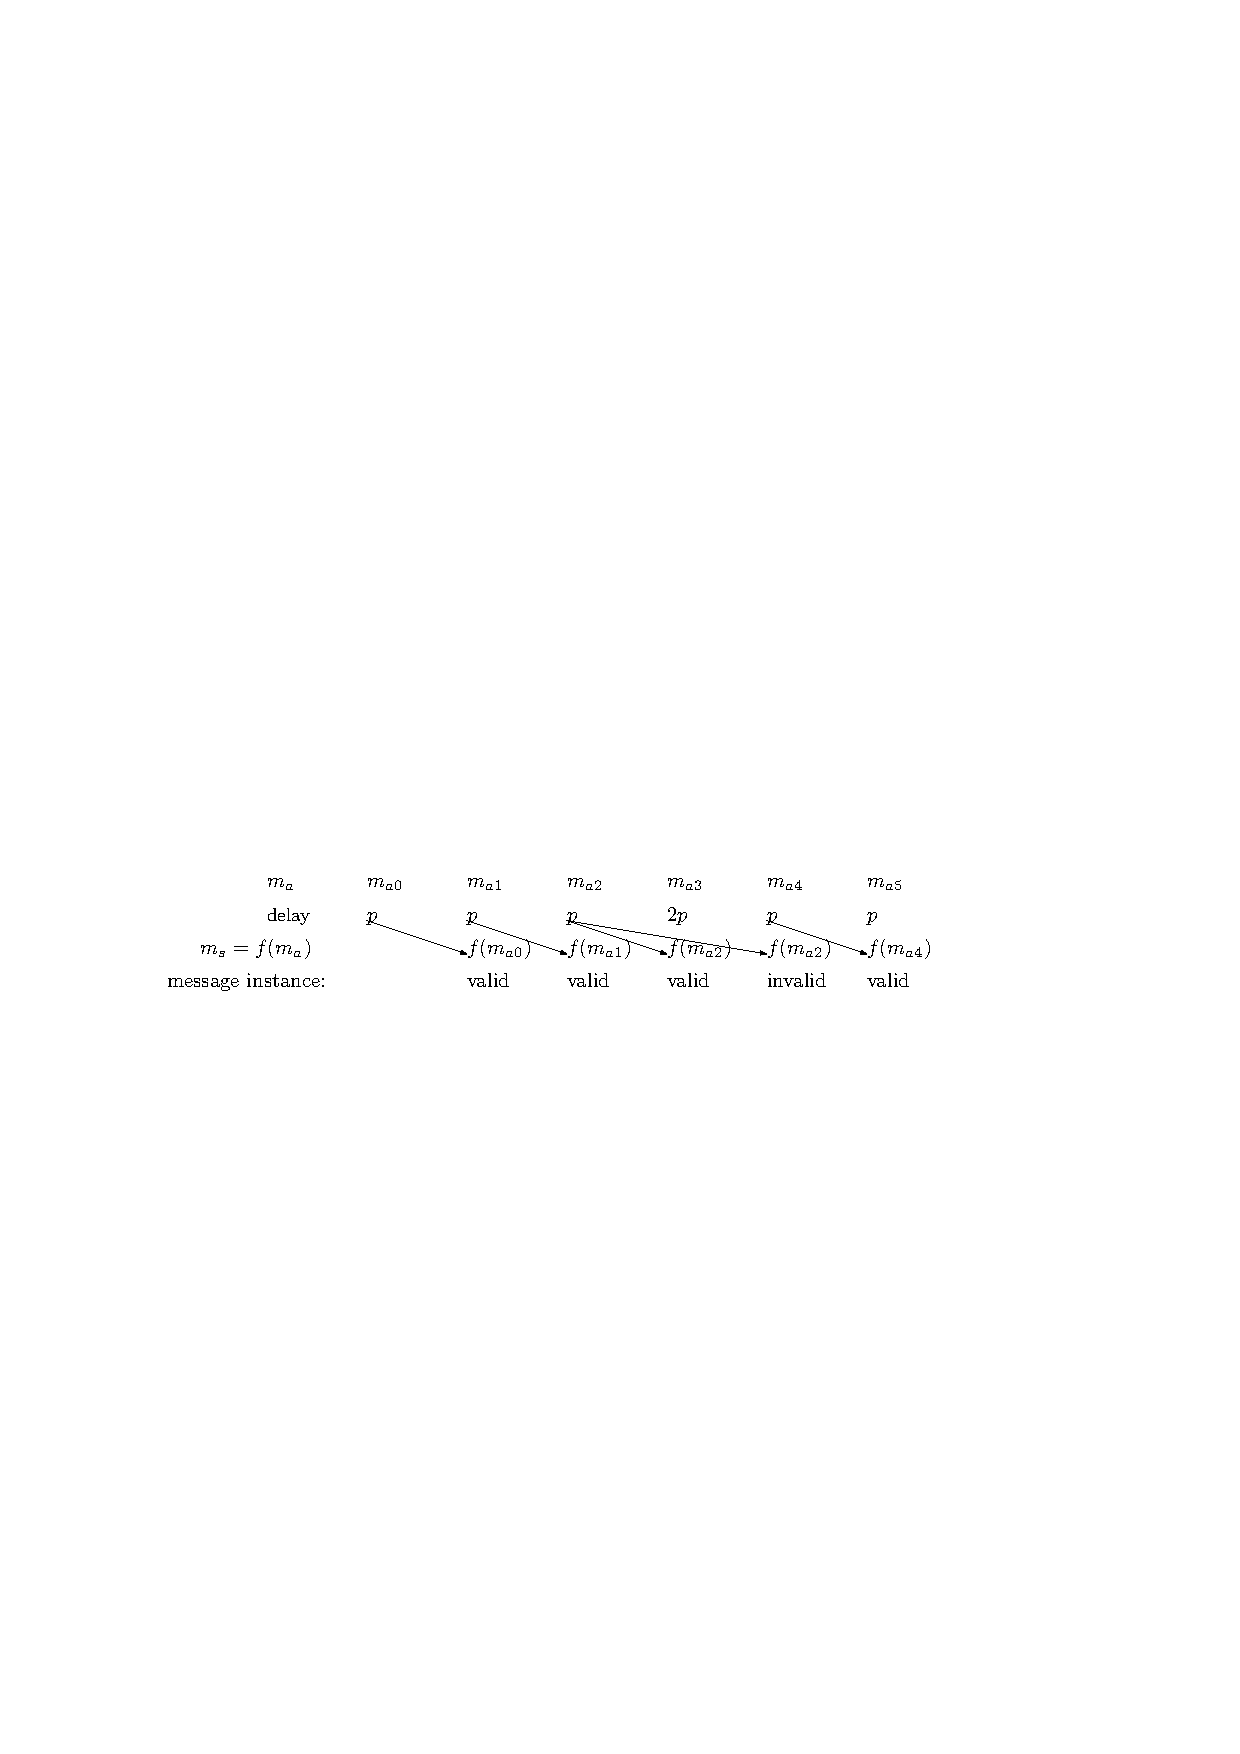
\includegraphics[width = 100mm]{timing_diagram_delay_cosntraint.pdf}
\end{center}
\caption{Timing diagram showing valid invalid sequence}
\label{tim_dig_delay}
\end{figure}

\begin{figure}
\begin{center}
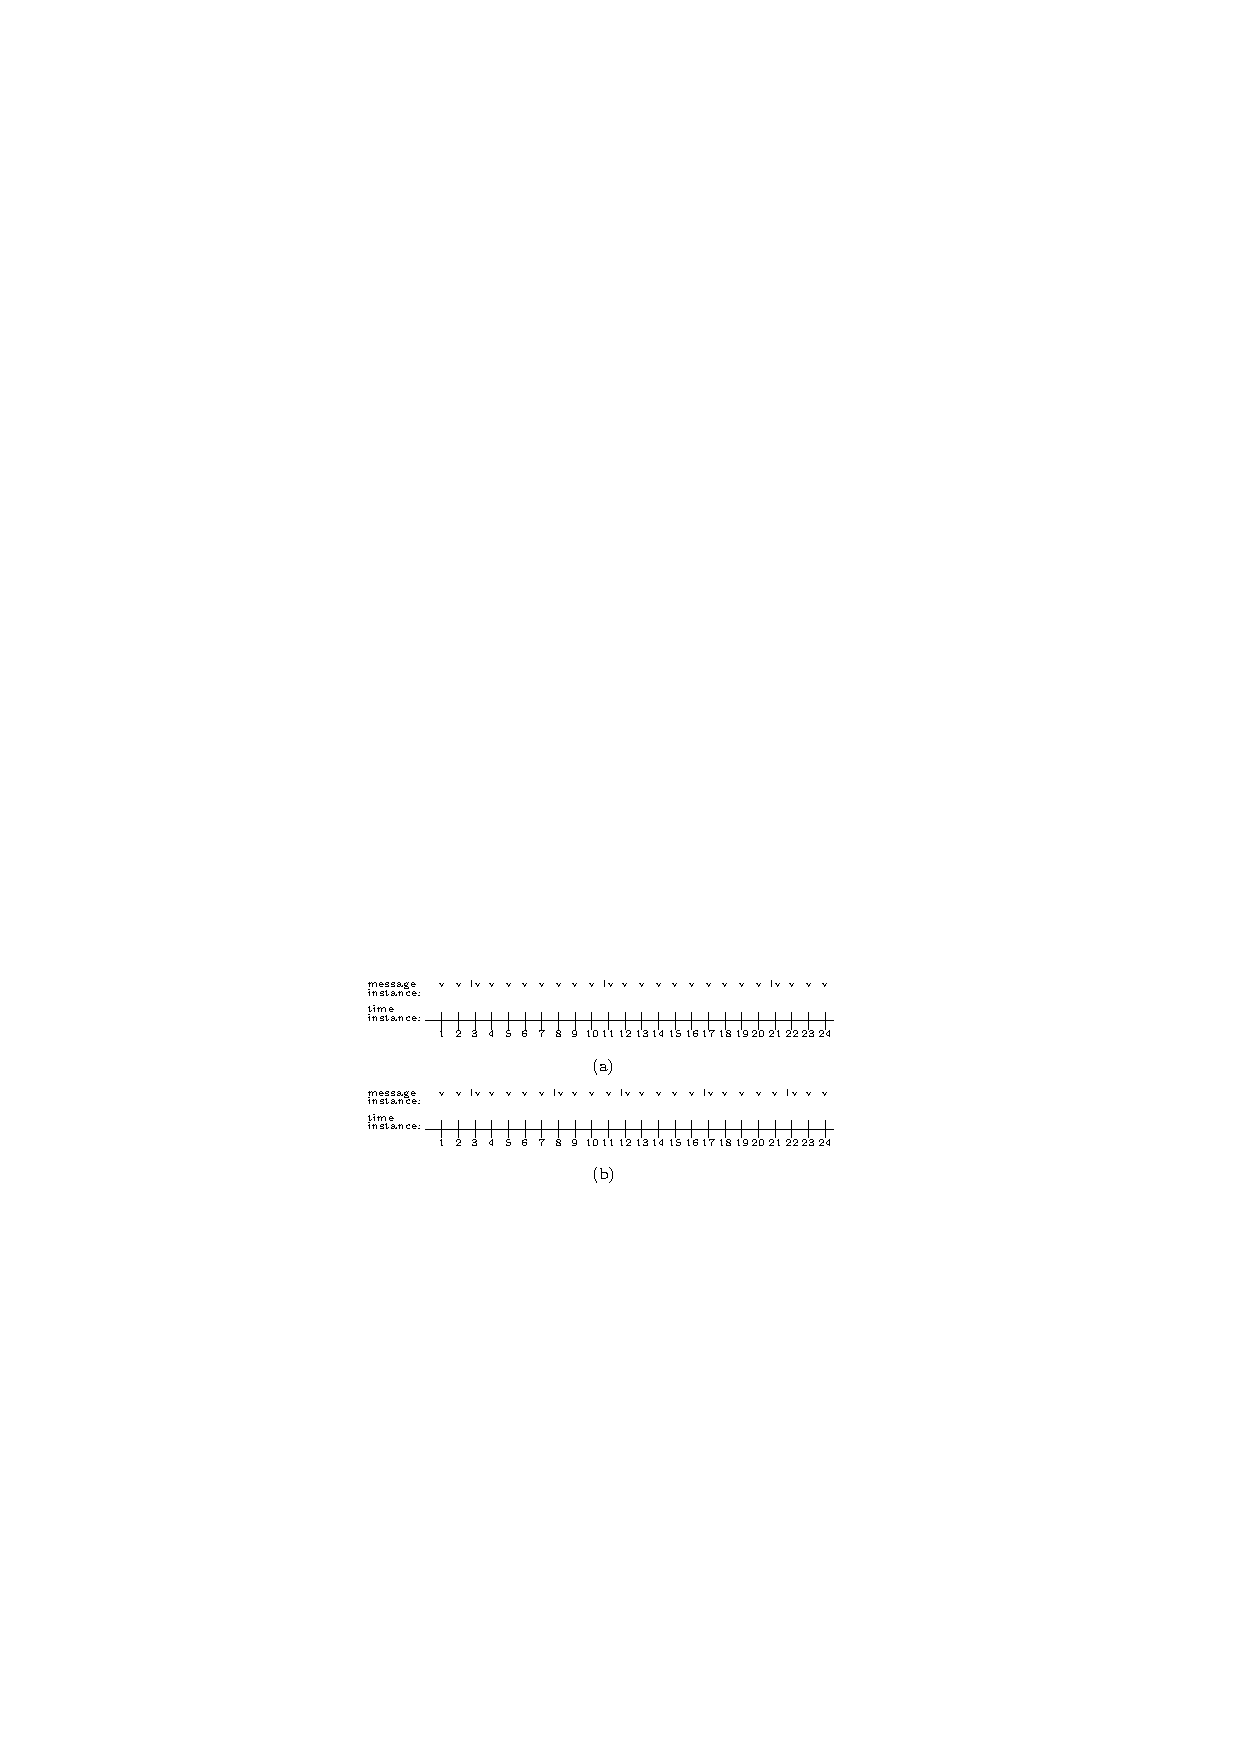
\includegraphics[width = 120mm]{valid_invalid.pdf}
\end{center}
\caption{Valid-Invalid messages from infinite sequence}
\label{tim_dig_cons}
\end{figure}


If a message is delivered within the particular period $p$ then it is called valid message but
if it is not delivered within $p$ period it becomes invalid. In the Fig.\ref{tim_dig_delay} we see that message
instance $m_{a3}$ requires $2p$ time period, so it does not get delivered within $p$ period and 
$m_{s2} = f(m_{a2})$ is delivered again which is now invalid.

In this problem model we are trying to demonstrate a system where an invalid message should 
followed by at least k valid messages. In Fig.\ref{tim_dig_cons}, we depicted the occurrence of invalid messages.
in Fig.\ref{tim_dig_cons}(a), invalid messages occurred after at least $k=6$ intervals but 
in Fig.\ref{tim_dig_cons}(b), invalid
messages occurred more frequently which will negatively impact the control performance.






